% !TeX spellcheck = da_DK
\subsection{Offsetjustering}
\subsubsection{Teori og design} \label{Offset_Teori_Design}
Det målte signal fra accelerometeret har et indbygget offset, som medfører, at outputtet ved $0$g påvirkning er halvdelen af accelerometerets spændingsforsyning. For at kunne forstærke signalet, der både skal indeholde positive og negative værdier, er det nødvendigt at justere offsettet. Dermed kan accelerometeret i steady state ved $0$g påvirkning have et outputsignal på $0$V. Måden hvorpå signalet centreres om $0$V er ved anvendelse af et differensforstærker kredsløb, som ses på \figref{fig:Differensforstaerker_generisk}. Dette kredsløb kan tage et inputsignal, kaldet $V_{b}$ på figuren, og fratrække et andet inputsignal, kaldet $V_{a}$ på figuren, der vil fungere som en referenceværdi.
\begin{figure}[H]
\centering
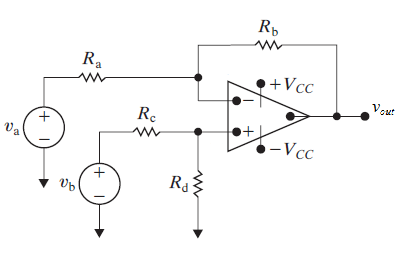
\includegraphics[scale=1.3]{figures/cProblemloesning/Differensforstaerker_generisk1.png}
\caption{På figuren ses et generisk differensforstærker kredsløb illustreret. Operationsforstærkeren vil trække inputtet $V_{a}$ fra inputtet $V_{b}$ og sende denne spænding ud i $V_{out}$. Hvorledes signalet forstærkes afhænger af værdierne for $R_{a}$, $R_{b}$, $R_{c}$ og $R_{d}$. \textit{(Revideret)} \cite{Nilsson2011}}
\label{fig:Differensforstaerker_generisk}
\end{figure}
\noindent Den ikke-inverterende terminals ($+V_{in}$) indgangsimpedans afhænger af $R_{c}$, hvorfor en buffer indsættes mellem outputsignalet fra forrige blok, som er accelerometeret, og blokken. Inputimpedansen i den inverterende terminal (-$V_{in}$) afhænger af modstanden $R_{a}$ på \figref{fig:Differensforstaerker_generisk} grundet det ikke-inverterende design, hvorfor der også indsættes en buffer, jævnfør afsnit \ref{spaendingsref_resultat} på side \pageref{spaendingsref_resultat}. \\
\noindent I \eqref{eq:Diff1} ses den simplificerede formel for differensforstærkerens kredsløb, hvor $\frac{R_a}{R_b} = \frac{R_c}{R_d}$; \cite{Nilsson2011}
\begin{equation}\label{eq:Diff1}
V_o = \frac{R_b}{R_a} \cdot (v_b - v_a)
\end{equation}
\noindent Der kan heraf ses, at forstærkningen på signalet kan bestemmes ved at vælge modstandene $R_a\text{ og }R_b$, og at det er spændingen $V_{a}$, der trækkes fra spændingen $V_{b}$. \\
I dette tilfælde kræves der ikke en forstærkning, hvorfor samtlige modstande skal have samme værdi. Da signalet ikke skal inverteres, sendes accelerometerets output ind i den ikke-inverterende terminal. Offsettet, som i dette tilfælde er en referenceværdi på $1.6325$V, sendes ind i den inverterende terminal. Dette illustreres på \figref{fig:Offset_generisk}:
\begin{figure}[H]
\centering
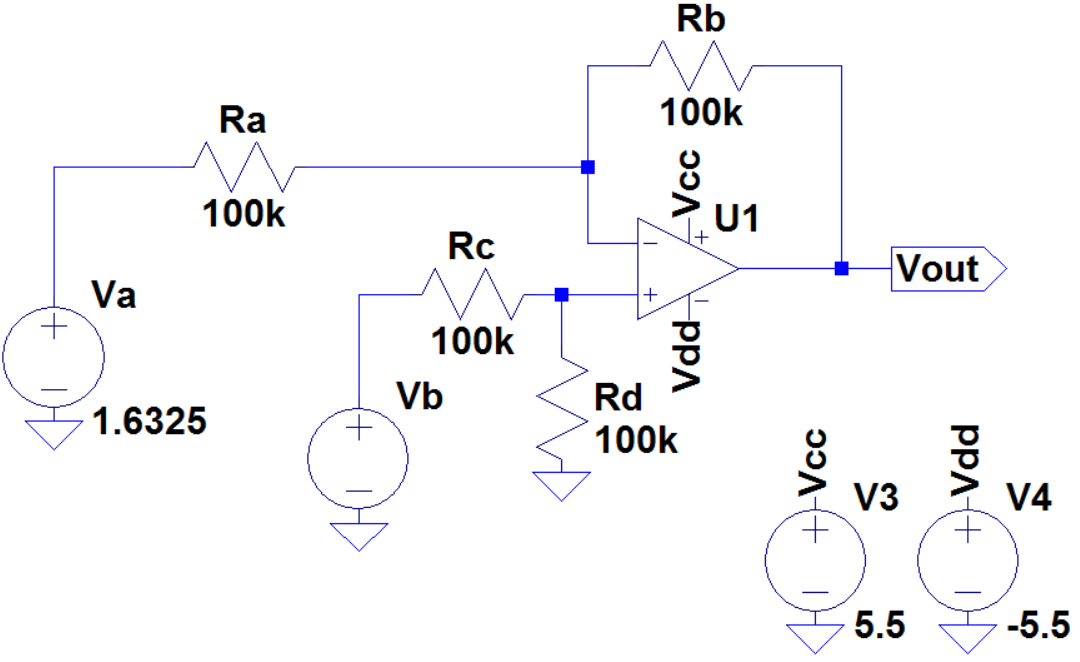
\includegraphics[scale=0.4]{figures/cProblemloesning/Offset_generisk.png}
\caption{På figuren ses offsetjusteringens opbygning. $V_{a}$ er referenceværdien, som sættes til $1.6325$V, og $V_{b}$ er outputtet fra accelerometeret, som vil skabe inputtet til operationsforstærkerens ikke-inverterende terminal. Modstandene i kredsløbet er ens, hvilket medfører at signalet ikke forstærkes, og spændingsforsyningen til operationsforstærkeren er $\pm5.5$V.}
\label{fig:Offset_generisk}
\end{figure}

\subsubsection{Simulering}
Der foretages tre simuleringer i LTspice - en for hhv. det højeste, middel og laveste output, fra accelerometret. Dette vil svare til $1$g påvirkning af accelerometerets x-akse og en $90^{\circ}$ rotation. Derudover foretages der en simulering for $0$g påvirkning, hvilket svarer til $0^{\circ}$ rotation. Resultaterne ses i \tableref{Tab:offset_sim}.
\begin{table}[H]
	\centering
	\begin{tabular}{|l|l|l|l|l|}
		\hline
		\multicolumn{1}{|c|}{\textit{Inputsignal}} & \multicolumn{1}{c|}{\textit{Offset}} & \multicolumn{1}{c|}{\textit{Forventet outputsignal}} & \multicolumn{1}{c|}{\textit{Simuleret outputsignal}} & \multicolumn{1}{c|}{\textit{Afvigelse}} \\ \hline
		$1.9638$V     & $1.6325$V    & $0.3313V$V    & $0.3313$V       & $0$\%              \\ \hline
		$1.6325$V     & $1.6325$V    & $0$V          & -$22.949\mu$V   & $\approx 0$\%      \\ \hline
		$1.3092$V     & $1.6325$V    & -$0.3233V$V   & -$0.3233$V      & $0$\%                \\ \hline
	\end{tabular}
	\caption{I tabellen ses resultaterne fra simuleringerne af offsettet for hhv. det højeste, middel og laveste input, som blokken kan modtage fra accelerometeret.}
	\label{Tab:offset_sim}
\end{table}
\noindent I tabellen fremgår det, at der er en lav afvigelse imellem de forventede og simulerede outputsignaler. Dette betyder, at kredsløbet fungerer rent teoretisk med ideelle komponenter. På \figref{fig:Offset_simulering} ses simuleringen af $1.6325$V input fra accelerometret.
 
\begin{figure}[H]
\centering
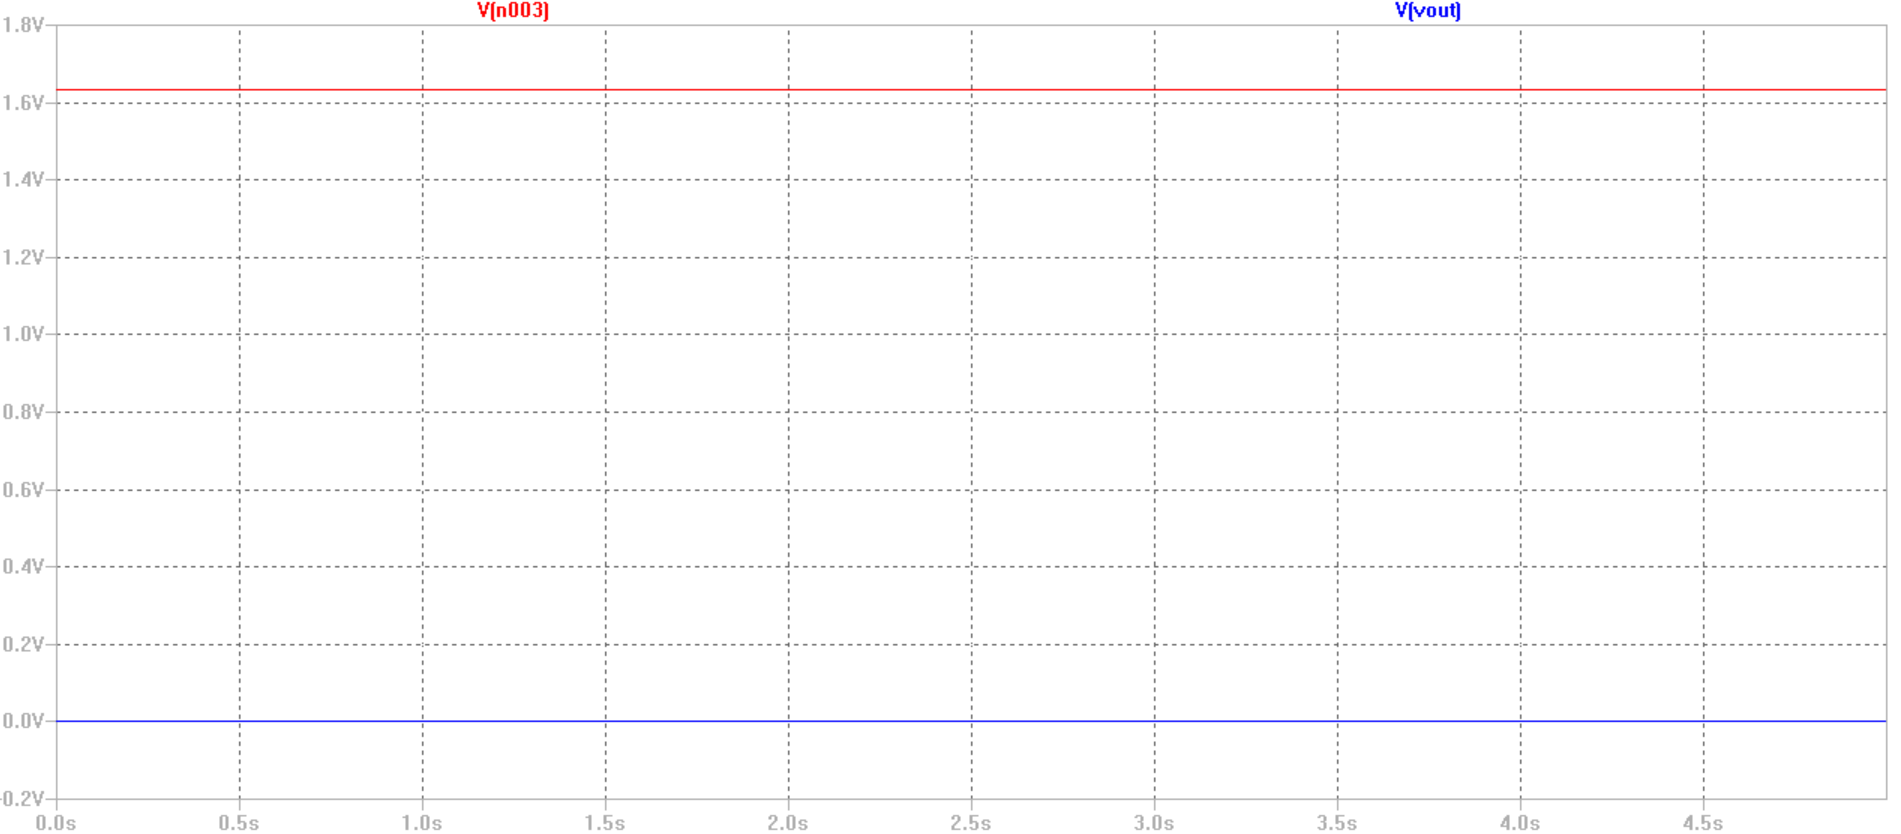
\includegraphics[scale=0.38]{figures/cProblemloesning/Offset_simulering.png}
\caption{På figuren ses en simulering af $1.6325$V input, hvilket giver et output på $\approx 0$V.}
\label{fig:Offset_simulering}
\end{figure}

\subsubsection{Implementering og test}
%I implementeringen bruges er reelle komponenter. Derfor antages der, at der kan være afvigelser fra resultaterne imellem simuleringen med ideelle komponenter og testen med reelle komponenter i implementeringen. \\
Der ses på \figref{fig:Offset_generisk}, at der skal benyttes fire modstande på $100$K$\Omega$ til opbygningen af offsettet. Resultatet af testen fremgår i \tableref{Tab:modstand_offset}.
\begin{table}[H]
	\centering
	\begin{tabular}{|l|l|l|}
		\hline
		\textit{Teoretisk} & \textit{Ved måling} & \textit{Afvigelse} \\ \hline
		$100$K$\Omega$       & $99.8$K$\Omega$       & $0.2$\%               \\ \hline
		$100$K$\Omega$       & $99.7$K$\Omega$       & $0.3$\%               \\ \hline
		$100$K$\Omega$       & $99.7$K$\Omega$       & $0.3$\%               \\ \hline
		$100$K$\Omega$       & $99.7$K$\Omega$       & $0.3$\%               \\ \hline
	\end{tabular}
	\caption{I tabellen ses, at alle fire modstande afviger lidt fra deres teoretiske værdi, hvilket er forventet af reelle komponenter. Kravet til disse fire modstande var, at de skulle være ens således at der ikke sker en forstærkning. Disse modstande accepteres derfor.}
	\label{Tab:modstand_offset}
\end{table}
\noindent Herefter implementeres kredsløbet. Til afbildning af signalet for de tre spændingsniveauer benyttes et multimeter. De aflæste resultater står under "Output" i \tableref{Tab:Offset_test}.
\begin{table}[H]
	\centering
	\begin{tabular}{l|l|l|l|l|l|}
		\cline{2-6}
		& \textit{\begin{tabular}[c]{@{}l@{}}Ønskede\\ input\end{tabular}} & \textit{Input} & \textit{\begin{tabular}[c]{@{}l@{}}Forventet\\ output\end{tabular}} & \textit{Output} & Afvigelse \\ \hline
		\multicolumn{1}{|l|}{\textit{\begin{tabular}[c]{@{}l@{}}$V_{a}$\\\end{tabular}}}    & $1.6325$V    & $1.6307$V    & $\times$    & $\times$   & $0.11\%$     \\ \hline
		\multicolumn{1}{|l|}{\multirow{2}{*}{\textit{\begin{tabular}[c]{@{}l@{}}$Vb$\\\end{tabular}}}} & $1.9638$V   & $1.9632$V    & $0.3325$V   & $0.3334$V   & $0.27\%$     \\ \cline{2-6} 
		\multicolumn{1}{|l|}{}   & $1.6346$V   & $1.6307$V    &  $0$V    & $1.008V$mV  & $\approx0\%$     \\ \cline{2-6} 
		\multicolumn{1}{|l|}{}   & $1.3092$V   &$1.3093X$V    & -$0.3214$V   & -$0.3204X$V     & $0.31\%$     \\ \hline
	\end{tabular}
	\caption{I tabellen ses en oversigt over de målte resultater for de tre spændingsniveauer.}
	\label{Tab:Offset_test}
\end{table}
\noindent I \tableref{Tab:Offset_test} betegner $Va$ referencespændingen, som sendes ind i den inverterende terminal. $Vb$ betegner det mindste, middel og største output, som accelerometret kan give ved $\pm90^{\circ}$ samt $0^{\circ}$. Derudover indsendes en spænding, som svarer til referencespændingen. Disse tre spændinger bliver sendt ind i den ikke-inverterende terminal. Det ønskede input er beregnet i afsnit \ref{Sec_Pilot_Data} på side \pageref{Sec_Pilot_Data} og burde være det, som sendes ind i $V2$. Input er den spænding, som sendes ind fra spændingsforsyningen og er målt med et multimeter. Forventet output udregnes ved at trække referencespændingens input fra det indsendte signal. Output er den afmålte værdi fra multimetret og afvigelsen kan derved beregnes. \\
Der ses i \tableref{Tab:Offset_test}, at afvigelserne ligger inde for tolerancen for offsettet beskrevet i afsnit \ref{OpsamlingsAfs} på side \pageref{OpsamlingsAfs}. Derfor anses disse afvigelser som acceptable, hvorfor offsetjusteringen i opsamlingsblokken accepteres.